\scanpage{174}
\figure{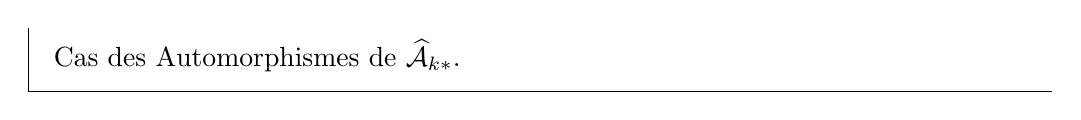
\begin{tikzpicture}
\node[anchor=west] at (.2,.45) {Cas des \uline{Automorphismes} de $\widehat{\mathcal A}_{k*}$.};
\draw (0,.8)--(0,0)--(13,0);
\end{tikzpicture}}

Nous nous intéressons maintenant aux automorphismes de la $k$-algèbre différentielle
$\tfrac12$-simpliciale $\mathcal A_{k*}=\mathcal A_*(k\{T\},k\{T\}^+,T)$.
Mais on \unsure{n'aura} de résultats simples qu'en complétant en
\[
 \widehat{\mathcal A}_{k*}\simeq(\widehat{\mathcal A}_{k,n})
\]
\[
 \begin{aligned}
 \widehat{\mathcal A}_{k,n}&\simeq k\{\{X_0,\ldots,X_n\}\}[dX_0,\ldots,dX_n]/(\textstyle\sum dX_i)\\
 &\simeq k\{\{T\}\}\{\{X_0,\ldots,X_n\}\}[dX_0,\ldots,dX_n]/
 (\textstyle\sum X_i-T,\sum dX_i)_{\mathrm{pd}}\\
 &\simeq k\{\{T\}\}\{\{X_0,\ldots,X_{n-1}\}\}[dX_0,\ldots,dX_{n-1}].
 \end{aligned}
\]

Les résultats sur les hom d'un tel $\widehat{\mathcal A}_{k,n}$ dans un
$\widehat{\mathcal A}_{k',n}$ sont les mêmes que tantôt [et peuvent s'exprimer en termes des
$\mathcal A_*(S,S^+,t)^\wedge$, (\unsure{où on fera} pour l'instant $S\simeq k\{\{T\}\}$),
avec
\[
 \mathcal A_n(S,S^+,t)^\wedge\simeq S\{\{X_0,\ldots,X_n\}\}[dX_0,\ldots,dX_n]
\]
mod idéal à p.d. engendré par $\sum X_i-t,\sum dX_i$
\[
 \simeq S\{\{X_0,\ldots,X_{n-1}\}\}[dX_0,\ldots,dX_{n-1}]\quad--
\]
mais $A'_1$ et les $B'_i$ $(i\geq1)$ sont dans
$\mathcal A_1(S,S^+,t)^\wedge\simeq S\{\{X_0\}\}$, au lieu de
$\unsure{S\{X_0\}|S\{\{X_0\}}$, i.e. les polynômes à p.d.
en $X_0$, coeff. en $S$, qui les exprimaient deviennent des séries à p.d. avec un
\margin{173}
